\documentclass{article}

\usepackage{amsmath, amssymb}
\usepackage{float}
\usepackage{graphicx}
\usepackage{subcaption}
\usepackage{color}

\usepackage{listings}


\definecolor{dkgreen}{rgb}{0,0.6,0}
\definecolor{gray}{rgb}{0.5,0.5,0.5}
\definecolor{mauve}{rgb}{0.58,0,0.82}

\lstset{frame=tb,
  language=python,
  aboveskip=3mm,
  belowskip=3mm,
  showstringspaces=false,
  columns=flexible,
  basicstyle={\small\ttfamily},
  numberstyle=\color{gray},
  keywordstyle=\color{blue},
  commentstyle=\color{dkgreen},
  stringstyle=\color{mauve},
  breaklines=true,
  breakatwhitespace=true,
  tabsize=3,
}
%

\addtolength{\topmargin}{-.875in}
\addtolength{\textheight}{1.75in}


\title{Project report - Week 2}

\begin{document}
	\maketitle
	\section{Introduction}
		To reduce over-fitting present in model training two methods were used: first, the training images were randomly modified using operations such as rotating, flipping or cropping, and second, the dropout layer was added to the model.
		With dropout active, randomly chosen neurons are ignored during specific training stage, which prevents building dependencies between neurons.
		Neurons are deactivated with probability $1 -p$.	
	\section{Results}
		\subsection{Artificial data generation}
			\begin{figure}[h!]
				\centering
				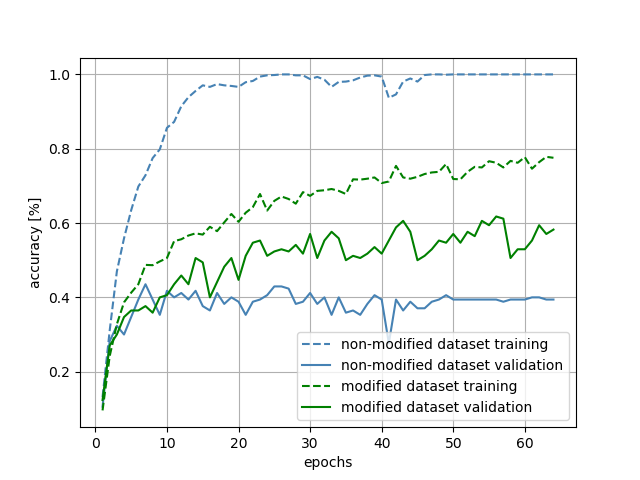
\includegraphics[width = \textwidth]{img/modified}
				\caption{Results of model training using dataset with and without modifications to images over 64 epochs.}		
			\end{figure}
			During training with non-modified dataset accuracy achieves its limit of accuracy (40\%) pretty fast, needing about 10 epochs. Over-fitting is clearly visible, with difference of accuracy between training and validation of 60 percentage points.
			In case of modified dataset training is slower, but it finishes with about 50\% better accuracy (60\%) and is less prone to over-fitting, with smaller difference between training and validation dataset.		
		\subsection{Dropout}
			\begin{figure}[h!]
				\centering				
				\caption{Accuracy for different values of $p$ after 64 epochs.}
				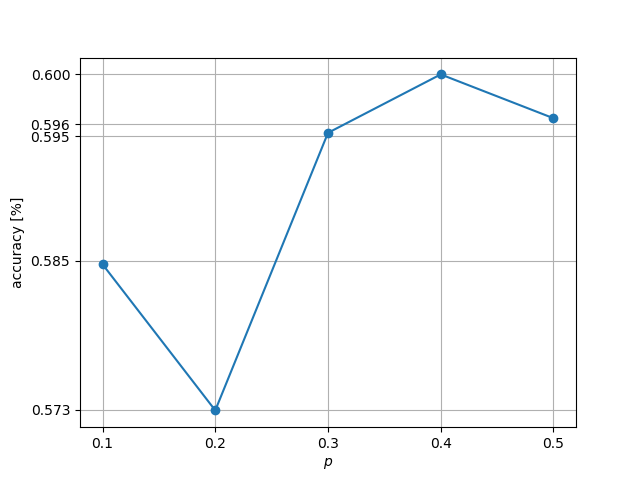
\includegraphics[width = \textwidth]{img/dropout}	
			\end{figure}
			While there isn't much difference between accuracy, $p = 0.4$ was chosen for the model as it gives the best result. 				
	\section{Summary}
		Use of artificial data generation and dropout layer allowed to achieve raise in accuracy of about 20 percentage points compared to model trained without those.
\end{document}